\documentclass[xcolor={dvipsnames,table},aspectratio=169]{beamer}
\usepackage[utf8]{inputenc}
\usepackage[T1]{fontenc}
\usepackage[brazil]{babel}
\usepackage{graphics,amssymb,amsfonts,amsmath}
\usepackage{tikz}
\usepackage{enumerate,hyperref}
\usepackage{palatino}
\usepackage{ragged2e}
\usepackage{minted}
\usepackage{booktabs}
\usepackage{verbatim}
\usepackage[export]{adjustbox}
\usepackage{tikz}                   
\usepackage{xcolor}
\usetikzlibrary{shadows}
\usetheme{AnnArbor}
\usecolortheme{orchid}
\usefonttheme[onlymath]{serif}

\newminted{java}{bgcolor=cyan!10}

\newcolumntype{C}[1]{>{\centering\let\newline\\\arraybackslash\hspace{0pt}}m{#1}}

\newcommand\setItemnumber[1]{\setcounter{enumi}{\numexpr#1-1\relax}}

\AtBeginSection[]{
  \begin{frame}
  \vfill
  \centering
  \begin{beamercolorbox}[sep=8pt,center,shadow=true,rounded=true]{title}
    \usebeamerfont{title}\insertsectionhead\par%
  \end{beamercolorbox}
  \vfill
  \end{frame}
}

\title[\sc{Tipos de Dados Fundamentais}]{Tipos de Dados Fundamentais}
\author[Roland Teodorowitsch]{Roland Teodorowitsch}
\institute[FPROG - EP - PUCRS]{Fundamentos de Programação - Escola Politécnica - PUCRS}
\date{17 de março de 2023}

\begin{document}
\justifying

%-------------------------------------------------------
\begin{frame}
	\titlepage
\end{frame}

%=======================================================
\section{Introdução}

%-------------------------------------------------------
\begin{frame}\frametitle{Objetivos}
\begin{itemize}
	\item declarar e inicializar variáveis e constantes
	\item entender as propriedades e limitações de números inteiros e de ponto-flutuante
	\item apreciar a importância de comentários e bons leiautes de código
	\item escrever expressões aritméticas e comandos de atribuição
	\item criar programas que leiam e processem entradas, e exibam os resultados
	\item aprender a usar o tipo String de Java
\end{itemize}
\end{frame}

%-------------------------------------------------------
\begin{frame}\frametitle{Conteúdos}
\begin{itemize}
	\item variáveis
	\item aritmética
	\item entrada e saída
	\item resolução de problemas: primeiro faça à mão
	\item cadeias de caracteres (\emph{strings})
\end{itemize}
\end{frame}

%=======================================================
\section{Variáveis}

%-------------------------------------------------------
\begin{frame}\frametitle{Variáveis}
\begin{itemize}
	\item a maioria dos programas de computador armazena valores temporários em locais de armazenamento identificados
	\begin{itemize}
		\item os programadores identificam estes locais para facilitar o acesso
	\end{itemize}
	\item exitem muitos tipos diferentes de armazenamento (com tamanhos diferentes) para guardar coisas diferentes
	\item você ``declara'' uma variável informando ao compilador:
	\begin{itemize}
		\item qual o tipo/tamanho da variável que você precisa
		\item por qual nome você quer se referir a ela
	\end{itemize}
\end{itemize}
\end{frame}

%-------------------------------------------------------
\begin{frame}[fragile]\frametitle{Declaração de Variáveis}
\begin{itemize}
	\item quando se declara uma variável, você frequentemente especifica um valor inicial para ela
	\item isto também é onde você diz ao compilador o tipo/tamanho que ela poderá armazenar
	\item por exemplo:\\~\\
\begin{javacode}
int latasPorPacote = 6;
\end{javacode}
	\begin{itemize}
		\item \texttt{int} é um tipo para números inteiros com sinal
		\item \texttt{double} é um tipo para números de ponto-flutuante e \texttt{String} é um tipo para textos
		\item use nomes de variáveis (\texttt{latasPorPacote}) sugestivos
		\item a atribuição de um valor inicial é opcional, mas geralmente é uma boa ideia
		\item uma declaração de variáveis termina por \texttt{;}
	\end{itemize}
\end{itemize}
\end{frame}

%-------------------------------------------------------
\begin{frame}\frametitle{Um exemplo: venda de refrigerantes}
\begin{itemize}
	\item Refrigerantes são vendidos em latas e garrafas. Uma loja oferece um pacote de 6 latas, cada lata com 355ml, pelo mesmo preço de uma garrafa de 2 litros. Qual você deve comprar? (1 litro = 1000 ml)
	\item Lista de variáveis:
	\begin{itemize}
		\item número de latas por pacote (valor inteiro)
		\item litros em uma garrafa (valor inteiro)
		\item litros em uma lata (valor fracionário)
	\end{itemize}
\end{itemize}
\begin{figure}[h]
	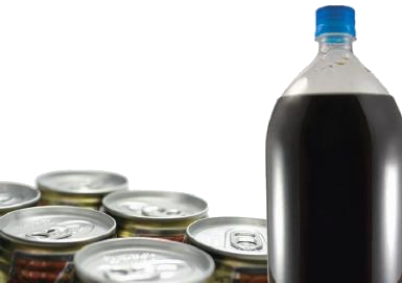
\includegraphics[height=0.3\paperheight,right]{pucrs-ep-fprog-unidade_02-tipos_de_dados_fundamentais-laminas-refrigerantes.png}
\end{figure}
\end{frame}

%-------------------------------------------------------
\begin{frame}[fragile]\frametitle{Variáveis e Conteúdos}
\begin{itemize}
	\item Você pode (opcionalmente) definir o conteúdo de uma variável quando você declara ela
\begin{javacode}
int latasPorPacote = 6;
\end{javacode}
	\item Uma variável é um local de armazenamento com um nome
	\item Imagine, por exemplo, uma vaga de estacionamento em um edifício-garagem:
	\begin{itemize}
		\item Identificador: J053
		\item Conteúdo: carro do João
	\end{itemize}
\end{itemize}
\begin{figure}[h]
	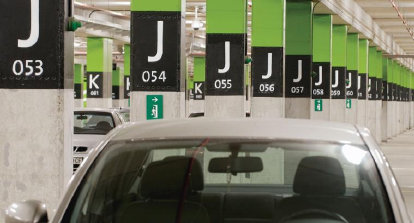
\includegraphics[height=0.3\paperheight,center]{pucrs-ep-fprog-unidade_02-tipos_de_dados_fundamentais-laminas-estacionamento.jpg}
\end{figure}
\end{frame}

%-------------------------------------------------------
\begin{frame}[fragile]\frametitle{Exemplos de Declaração de Variáveis em Java}
{\footnotesize
\begin{center}
\begin{tikzpicture}
\node[drop shadow,fill=white,inner sep=0pt] 
{\rowcolors{1}{RoyalBlue!20}{RoyalBlue!5}
  \begin{tabular}{|c|l|p{6cm}|}
\hline
    \textbf{V/F} & \textbf{Código} & \textbf{Descrição}\\
\hline
    \textcolor{green}{\textbf{V}} & \texttt{int latas = 6;}                & Declara uma variável inteira e inicializa ela com 6\\
    \textcolor{green}{\textbf{V}} & \texttt{int total = latas + garrafas;} & O valor inicial não precisa ser um valor fixo. (Naturalmente, \texttt{latas} e \texttt{garrafas} devem ter sido declarados e inicializados.)\\
    \textcolor{red}{\textbf{X}} & \texttt{garrafas = 1;}                   & \textbf{ERRO:} está faltando o tipo. Esta expressão não é uma declaração, mas a atribuição de um novo valor para a variável.\\
    \textcolor{red}{\textbf{X}} & \texttt{int volume="2";}                 & \textbf{ERRO:} você não pode inicializar um número com um \emph{string}\\
    \textcolor{green}{\textbf{V}} & \texttt{int latasPorPacote;}           & Declara uma variável inteira sem inicializá-la. Isto pode causar erros. \\
    \textcolor{green}{\textbf{V}} & \texttt{int reais, centavos;}          & Declara 2 variáveis inteiras em uma sentença.\\
\hline
  \end{tabular}
};
\end{tikzpicture}
\end{center}
}
\end{frame}

%-------------------------------------------------------
\begin{frame}[fragile]\frametitle{Por quê há diferentes tipos?}
\begin{itemize}
	\item Há 3 tipos diferentes de variáveis que usaremos neste capítulo
	\begin{enumerate}
		\item um número inteiro (sem parte fracionária): \textbf{\texttt{int}}
		\item um número com parte fracionária: \textbf{\texttt{double}}
		\item uma palavra (um grupo de caracteres): \textbf{\texttt{String}}
	\end{enumerate}
	\item Especifique o tipo antes do nome nas declarações:
\begin{javacode}
int latasPorPacote = 6;
double volumeLata = 0.355;
\end{javacode}
\end{itemize}
\end{frame}

%-------------------------------------------------------
\begin{frame}\frametitle{Por quê há diferentes tipos?}
\begin{itemize}
	\item De volta à analogia do edifício-garagem, existem espaços diferentes para diferentes tipos de veículos
	\begin{itemize}
		\item bicicleta
		\item motocicleta
		\item carros grandes
		\item carros compactos
	\end{itemize}
\end{itemize}
\end{frame}

%-------------------------------------------------------
\begin{frame}[fragile]\frametitle{Constantes Numéricas em Java}
\begin{itemize}
	\item Algumas vezes quando você digita um número, o compilador tem que ``adivinhar'' de qual tipo ele é
{\scriptsize
\begin{javacode}
amt = 6 * 12.0;
PI = 3.14;
volLata = 0.335;
\end{javacode}
}
\end{itemize}
{\scriptsize
\begin{center}
\begin{tikzpicture}
\node[drop shadow,fill=white,inner sep=0pt] 
{\rowcolors{1}{RoyalBlue!20}{RoyalBlue!5}
  \begin{tabular}{|c|l|l|p{10cm}|}
\hline
    ~ & \textbf{Número} & \textbf{Tipo} & \textbf{Comentário}\\
\hline
    \textcolor{green}{\textbf{V}} & \texttt{6}       & \texttt{int}    & Um inteiro não tem parte fracionária.\\
    \textcolor{green}{\textbf{V}} & \texttt{-6}      & \texttt{int}    & Inteiros podem ser negativos.\\
    \textcolor{green}{\textbf{V}} & \texttt{0}       & \texttt{int}    & Zero é um inteiro.\\
    \textcolor{green}{\textbf{V}} & \texttt{0.5}     & \texttt{double} & Um número com parte fracionária é do tipo \texttt{double}.\\
    \textcolor{green}{\textbf{V}} & \texttt{1.0}     & \texttt{double} & Um inteiro com parte fracionária \texttt{.0} é do tipo \texttt{double}.\\
    \textcolor{green}{\textbf{V}} & \texttt{1E6}     & \texttt{double} & Um número em notação exponencial: $1 \times 10^6$ ou $1000000$. Números em notação exponencial sempre são do tipo \texttt{double}.\\
    \textcolor{green}{\textbf{V}} & \texttt{2.96E-2} & \texttt{double} & Expoente negativo: $2.96 \times 10^{-2} = 2.96 / 100 = 0.0296$.\\
    \textcolor{red}{\textbf{X}}   & \texttt{100,000} & ~               & \textbf{ERRO:} não use vírgula como separador ou ponto decimal.\\
    \textcolor{red}{\textbf{X}}   & \texttt{3 1/2}   & ~               & \textbf{ERRO:} não use frações, use a notação decimal (3.5).\\
\hline
  \end{tabular}
};
\end{tikzpicture}
\end{center}
}
\end{frame}

%-------------------------------------------------------
\begin{frame}\frametitle{Números em Ponto-Flutuante}
\begin{itemize}
	\item Java armazena números com partes fracionárias como números de ponto-flutuante
	\item Eles são armazenados em quatro partes
	\begin{itemize}
		\item Sinal
		\item Mantissa
		\item Base
		\item Expoente
	\end{itemize}
	\item Por exemplo: $-5 \times 10^{0}$
	\item Um \texttt{double} é um número de dupla precisão: ele ocupa 2 vezes o espaço de armazenamento (mantissa de 52 bits) do que o \texttt{float} (mantissa de 23 bits).
\end{itemize}
\end{frame}

%-------------------------------------------------------
\begin{frame}\frametitle{Nomes de Variáveis}
\begin{itemize}
	\item Os nomes deveriam descrever o propósito da variável
	\item Use estas regras simples
	\begin{enumerate}
		\item Nomes de variáveis devem iniciar com uma letra, com o caractere ``sublinhado'' (\texttt{\_}) ou com o caractere ``cifrão'' (\texttt{\$}), e continuar com letras (maiúsculas ou minúsculas), dígitos, sublinhado ou cifrão
		\item Você não pode usar outros símbolos (\texttt{?}, \texttt{\%}, etc.), nem espaço.
		\item Separe palavras com a notação ``camelHump'': comece com minúsculas e use letras maiúsculas para marcar a separação de palavras
		\item Não use palavras-reservadas de Java
	\end{enumerate}
\end{itemize}
\end{frame}

%-------------------------------------------------------
\begin{frame}\frametitle{Nomes de Variáveis Legais e Ilegais em Java}
{\footnotesize
\begin{center}
\begin{tikzpicture}
\node[drop shadow,fill=white,inner sep=0pt] 
{\rowcolors{1}{RoyalBlue!20}{RoyalBlue!5}
  \begin{tabular}{|c|l|p{10cm}|}
\hline
    ~ & \textbf{Nome de variável}  & \textbf{Comentário}\\
\hline
    \textcolor{green}{\textbf{V}}  & \texttt{volLata1}  & Nomes de variáveis consistem de letras, números e sublinhado.\\
    \textcolor{green}{\textbf{V}}  & \texttt{x}         & Em matemática, usa-se nomes curtos de variáveis, tal como $x$ ou $y$. Eles são permitidos em Java, mas não são muito comuns, pois eles tornam o programa mais difícil de entender.\\
    \textcolor{yellow}{\textbf{!}} & \texttt{VolLata}   & \textbf{Atenção:} Java distingue maiúsculas de minúsculas. Este nome de variável é diferente de \texttt{volLata}, e viola a convenção de se inicar nomes de variáveis com minúsculas.\\
    \textcolor{red}{\textbf{X}}    & \texttt{6latas}    & \textbf{Erro:} Nomes de variáveis não podem iniciar com números.\\
    \textcolor{red}{\textbf{X}}    & \texttt{vol lata}  & \textbf{Erro:} Nomes de variáveis não podem conter espaços.\\
    \textcolor{red}{\textbf{X}}    & \texttt{double}    & \textbf{Erro:} Você não pode usar palavras-reservadas como nome de variáveis.\\
    \textcolor{red}{\textbf{X}}    & \texttt{lit/pac.l} & \textbf{Erro:} Você não pode usar símbolos como \texttt{/} ou \texttt{.}.\\
\hline
  \end{tabular}
};
\end{tikzpicture}
\end{center}
}
\end{frame}

%-------------------------------------------------------
\begin{frame}[fragile]\frametitle{Expressões de Atribuição}
\begin{itemize}
	\item Use a ``expressão de atribuição'' (com um \texttt{=}) para colocar um novo valor em uma variável
\begin{javacode}
int latasPorPacote = 6;  // declara e inicializa
latasPorPacote = 12;     // atribui
\end{javacode}
	\item Cuidado: o sinal \texttt{=} \textbf{NÃO} é usado para comparações
	\begin{itemize}
		\item Ele copia o valor calculado no lado direito da expressão para a variável que está à sua esquerda.
		\item Aprenderemos sobre comparações mais tarde
	\end{itemize}
\end{itemize}
\end{frame}

%-------------------------------------------------------
\begin{frame}[fragile]\frametitle{Sintaxe da Atribuição}
\begin{itemize}
	\item O valor calculado no lado direito do operador de atribuição (\texttt{=}) é copiado para a variável que está à sua esquerda
\begin{javacode}
double total = 0;   /* Isto e' a inicializacao
                       de uma nova variavel e
                       nao uma atribuicao */
...
// Isto e' uma atribuicao
total = garrafas * VOLUME_GARRAFA;
...
// O mesmo nome pode aparecer nos dois lados de uma atribuicao
total = total + latas * VOLUME_LATA;
\end{javacode}
\end{itemize}
\end{frame}

%-------------------------------------------------------
\begin{frame}\frametitle{Atualização de uma Variável}
Passo-a-passo: \texttt{volumeTotal = volumeTotal + 2;}
\begin{enumerate}
	\item Calcule o lado direito da atribuição. Encontre o valor de \texttt{volumeTotal}, e adicione 2 a ele
	\item Armazene o resultado na variável indicada no lado esquerdo do operador de atribuição (neste caso, \texttt{totalVolume})
\end{enumerate}
\end{frame}

%-------------------------------------------------------
\begin{frame}[fragile]\frametitle{Constantes}
\begin{itemize}
	\item Quando uma variável é definida com a palavra-reservada \texttt{final}, o seu valor não poderá ser alterado
\begin{javacode}
final double VOLUME_GARRAFA = 2;
\end{javacode}
	\item É uma boa prática usar constantes rotuladas para explicar valores a serem usados em cálculos
	\begin{itemize}
		\item Qual forma é mais clara?
\begin{javacode}
double volumeTotal = garrafas * 2;
double volumeTotal = garrafas * VOLUME_GARRAFA;
\end{javacode}
	\end{itemize}
	\item Um programador lendo a primeira senteça pode não entender o significado de 2
	\item Da mesma forma, se a constante for usada em vários lugares e necessitar ser alterada, bastará alterar a inicialização
\end{itemize}
\end{frame}

%-------------------------------------------------------
\begin{frame}[fragile]\frametitle{Declaração de Constantes}
\begin{itemize}
	\item A palavra-reservada \texttt{final} indica que o valor não poderá ser modificado
	\item por exemplo:\\~\\
\begin{javacode}
final double VOLUME_LATA = 0.355; // Litros em uma lata
\end{javacode}
	\begin{itemize}
		\item Não é obrigatório, mas costuma-se usar letras maiúsculas para constantes
		\item O comentário explica como o valor da constante foi definido
	\end{itemize}
\end{itemize}
\end{frame}

%-------------------------------------------------------
\begin{frame}[fragile]\frametitle{Comentários em Java}
\begin{itemize}
	\item Lembre-se: há 3 tipos de comentários em Java
{\scriptsize
\begin{javacode}
// Comentario de uma unica linha

/*
   Comentario de multiplas linhas
*/

/**
   Comentarios JavaDoc
   @author Aqui Vai o Seu Nome
   @version 15 ago. 2022
*/
\end{javacode}
}
	\item O compilador ignora comentários (comentários JavaDoc geram documentação)
	\item Identifique assunto, autoria e versão em um comentário JavaDoc em cada programa
	\item Use comentários para adicionar explicações para facilitar o entendimento do código
\end{itemize}
\end{frame}

%-------------------------------------------------------
\begin{frame}[fragile]\frametitle{Exemplo de Programa Comentado em Java}
{\footnotesize
\begin{javacode}
/**
   Este programa calcula o volume (em litros) de um pacote de
   6 latas de refrigerante e de uma garrafa de 2 litros de refrigerante
*/

public class Volume1 {
  public static void main(String[] args) {
    int latasPorPacote = 6;
    final double VOLUME_LATA = 0.355; // Litros em uma lata
    double volumeTotal = latasPorPacote * VOLUME_LATA;

    System.out.print("Um pacote de 6 latas de refrigerante contem ");
    System.out.print(volumeTotal);
    System.out.println(" litros.");
  }
}
\end{javacode}
}
\end{frame}

%-------------------------------------------------------
\begin{frame}[fragile]\frametitle{Erros Comuns}
\begin{itemize}
	\item Variáveis não delcaradas
	\begin{itemize}
		\item Você deve declarar as variáveis antes de usá-las: (ou seja, acima no código)
\begin{javacode}
double volumeLatas = 6 * litrosPorLata; // ??
double litrosPorLata = 0.355;
\end{javacode}
	\end{itemize}
	\item Variáveis não inicializadas
	\begin{itemize}
		\item Você deve inicializar as variáveis (isto é, definir um conteúdo para elas) antes de usá-las
\begin{javacode}
int garrafas;
int volumeGarrafas = garrafas * 2; // ??
\end{javacode}
	\end{itemize}
\end{itemize}
\end{frame}

%-------------------------------------------------------
\begin{frame}[fragile]\frametitle{Erros Comuns}
\begin{itemize}
	\item \emph{Overflow} significa que a área de armazenamento da variável não pode guardar o valor
\begin{javacode}
int cinquentaMilhoes = 50000000;
System.out.println(100 * cinquentaMilhoes);
// Esperava-se 5000000000
\end{javacode}
	\item Será impresso 705032704
	\item Por quê?
	\begin{itemize}
		\item O resultado (5 bilhões) estourou a capacidade de uma variável \texttt{int}
		\item O valor máximo para um \texttt{int} é \textbf{+2,147,483,647}
	\end{itemize}
	\item Use um \texttt{long} em vez de um \texttt{int} (ou um \texttt{double})
\end{itemize}
\end{frame}

%-------------------------------------------------------
\begin{frame}[fragile]\frametitle{Erros Comuns}
\begin{itemize}
	\item Erros de arredondamento: valores de ponto-flutuante não são exatos (isto é uma limitação da conversão entre decimal e binário)
\begin{javacode}
double preco = 4.35;
double quantidade = 100;
double total = preco * quantidade;
// Deveria ser 100 * 4.35 = 435.00
System.out.println(total); // Imprime 434.99999999999999
\end{javacode}
	\item Você pode lidar com erros deste tipo arredondando o valor para o inteiro mais próximo ou exibindo um número fixo de dígitos após o ponto decimal.
\end{itemize}
\end{frame}

%-------------------------------------------------------
\begin{frame}\frametitle{Tipos Numéricos em Java}
\begin{itemize}
	\item Tipos Inteiros
	\begin{itemize}
		\item \texttt{byte}: um número muito pequeno de 1 byte ou 8 bits (-128 to +127)
		\item \texttt{short}: um número pequeno (-32768 to +32767)
		\item \texttt{int}: um número grande (-2,147,483,648 ou \texttt{Integer.MIN\_VALUE} até +2,147,483,647 ou \texttt{Integer.MAX\_VALUE})
		\item \texttt{long}: um número muito grande, com aproximadamente 19 dígitos decimais
	\end{itemize}
	\item Tipos de Ponto-Flutuante
	\begin{itemize}
		\item \texttt{float}: um número fracionário de precisão simples com cerca de 7 casas decimais e intervalo aproximado de $\pm 10^{38}$
		\item \texttt{double}: um número fracionário de dupla precisão, para matemática pesada, com cerca de 15 casa decimais e intervalo aproximado de $\pm 10^{308}$
	\end{itemize}
	\item Outros Tipos
	\begin{itemize}
		\item \texttt{boolean}: \texttt{true} (verdadeiro) ou \texttt{false} (falso)
		\item \texttt{char}: um símbolo ou caracter na codificação Unicode
	\end{itemize}
\end{itemize}
\end{frame}

%-------------------------------------------------------
\begin{frame}\frametitle{Armazenamento (em Bytes) por Tipo}
\begin{itemize}
	\item Tipos Inteiros
	\begin{itemize}
		\item \texttt{byte}: 1 byte
		\item \texttt{short}: 2 bytes
		\item \texttt{int}: 4 bytes
		\item \texttt{long}: 8 bytes
	\end{itemize}
	\item Tipos de Ponto-Flutuante
	\begin{itemize}
		\item \texttt{float}: 4 bytes
		\item \texttt{double}: 8 bytes
	\end{itemize}
	\item Outros Tipos
	\begin{itemize}
		\item \texttt{boolean}: 1 bit
		\item \texttt{char}: 2 bytes
	\end{itemize}
\end{itemize}
\end{frame}

%=======================================================
\section{Aritmética}

%-------------------------------------------------------
\begin{frame}\frametitle{Aritmética}
\begin{itemize}
	\item Java suporta as mesmas operações básicas que uma calculadora
	\begin{itemize}
		\item parênteses
		\item operadores unários (sinal): $-a$, $+a$
		\item operadores binários: multiplicação ($a*b$), divisão inteira ou real ($a/b$), resto da divisão inteira ($a\%b$), adição ($a+b$), subtração ($a-b$)
	\end{itemize}
	\item Porém, as expressões devem escritas de uma forma diferente:
	\begin{itemize}
		\item Em Álgebra: \[x = \frac{a+b}{2}\]
		\item Em Java: ~ ~ ~ ~\texttt{x = (a + b) / 2.0;}
	\end{itemize}
	\item A precedência nas expressões em Java é similar à precedência da Álgebra:
	\begin{itemize}
		\item Parenteses, Operadores Unários, Multiplicação/Divisão/Resto, Soma/Subtração
		\item Em caso de empate: resolver da esquerda para a direita
	\end{itemize}
\end{itemize}
\end{frame}

%-------------------------------------------------------
\begin{frame}[fragile]\frametitle{Divisão Inteira e Resto da Divisão Inteira}
\begin{itemize}
	\item Quando ambas as partes de uma divisão são inteiras, o resultado será um inteiro
	\begin{itemize}
		\item Toda informação fracionária será perdida e o resultado não será arredondado
\begin{javacode}
int resultado = 7 / 4;
\end{javacode}
		\item O valor de \texttt{resultado} será 1
	\end{itemize}
	\item Se você estiver interessado no resto da divisão de dois inteiros, use o operador \texttt{\%} (chamado módulo)
	\begin{itemize}
		\item Por exemplo, para:
\begin{javacode}
int resto = 7 % 4;
\end{javacode}
		\item O valor de \texttt{resto} será 3
		\item O resto da divisão também é chamado de módulo da divisão
	\end{itemize}
\end{itemize}
\end{frame}

%-------------------------------------------------------
\begin{frame}[fragile]\frametitle{Exemplos de Divisão Inteira e Resto da Divisão Inteira}
{\footnotesize
\begin{center}
\begin{tikzpicture}
\node[drop shadow,fill=white,inner sep=0pt] 
{\rowcolors{1}{RoyalBlue!20}{RoyalBlue!5}
  \begin{tabular}{|p{2.5cm}|c|p{10cm}|}
\hline
    \textbf{Express\~ao (onde n=1729)}  & \textbf{Valor} & \textbf{Comentário}\\
\hline
    \texttt{n \% 10}   & \texttt{9}     & \texttt{n \% 10} é sempre o último dígito de \texttt{b}\\
    \texttt{n / 10}    & \texttt{172}   & Isto será sempre \texttt{n} sem o último dígito\\
    \texttt{n \% 100}  & \texttt{29}    & Os últimos 2 dígitos de \texttt{n}\\
    \texttt{n / 10.0}  & \texttt{172.9} & Como \texttt{10.0} é um número em ponto-flutuante, a parte fracionária não é descartada\\
    \texttt{-n \% 10}  & \texttt{-9}    & Como o primeiro número é negativo, o resto também é\\
    \texttt{n \% 2}    & \texttt{1}     & \texttt{n \% 2} é \texttt{0} se \texttt{n} for par, \texttt{1} ou \texttt{-1} se \texttt{n} for ímpar\\
\hline
  \end{tabular}
};
\end{tikzpicture}
\end{center}
}

\begin{itemize}
	\item Isto é muito útil para calcular troco
\begin{javacode}
int totalCentavos = 1729;
int reais = totalCentavos / 100;      // 17
int centavos = totalCentavos % 100;   // 29
\end{javacode}
\end{itemize}
\end{frame}

%-------------------------------------------------------
\begin{frame}\frametitle{Potências e Raízes}
\begin{itemize}
	\item Em Java, não há símbolos para potência e raiz
	\item Por exemplo, \[b \times \left(1+\frac{r}{100}\right)^n\]
	\item Será implementado como: \texttt{b * Math.pow(1 + r / 100, n)}
\begin{figure}[h]
	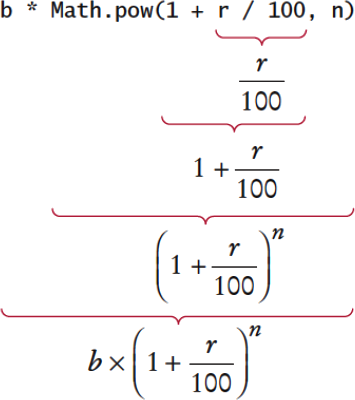
\includegraphics[height=0.3\paperheight,center]{pucrs-ep-fprog-unidade_02-tipos_de_dados_fundamentais-laminas-pow.png}
\end{figure}
	\item Em Java, a classe \texttt{Math} disponibiliza uma série de funções matemáticas
\end{itemize}
\end{frame}

%-------------------------------------------------------
\begin{frame}\frametitle{Métodos Matemáticos}
{\footnotesize
\begin{center}
\begin{tikzpicture}
\node[drop shadow,fill=white,inner sep=0pt] 
{\rowcolors{1}{RoyalBlue!20}{RoyalBlue!5}
  \begin{tabular}{|c|p{10cm}|}
\hline
    \textbf{Método}  & \textbf{Retorna}\\
\hline
    \texttt{Math.sqrt(x)}      & Raiz quadrada de $x$ ($\ge 0$)\\
    \texttt{Math.pow(x, y)}    & $x^y$\\
    \texttt{Math.sin(x)}       & Seno de $x$ ($x$ em radianos)\\
    \texttt{Math.cos(x)}       & Cosseno de $x$ ($x$ em radianos)\\
    \texttt{Math.tan(x)}       & Tangente de $x$ ($x$ em radianos)\\
    \texttt{Math.toRadians(x)} & Converte $x$ graus para radianos (isto é, retorna $x \cdot \pi / 180)$\\
    \texttt{Math.toDegrees(x)} & Converte $x$ radianos para graus (isto é, retorna $x \cdot 180 / \pi$)\\
    \texttt{Math.exp(x)}       & $e^x$\\
    \texttt{Math.log(x)}       & Logaritmo natural ($\ln(x)$, $x > 0$)\\
    \texttt{Math.log10(x)}     & Logaritmo decimal ($\log_{10}(x)$, $x > 0$)\\
    \texttt{Math.round(x)}     & Inteiro mais próximo de $x$ (como um \texttt{long})\\
    \texttt{Math.abs(x)}       & Absolute value $\left|x\right|$\\
    \texttt{Math.max(x, y)}    & O maior valor entre $x$ e $y$\\
    \texttt{Math.min(x, y)}    & O menor valor entre $x$ e $y$\\
    ... & ...\\
\hline
  \end{tabular}
};
\end{tikzpicture}
\end{center}
}	
\end{frame}

%-------------------------------------------------------
\begin{frame}[fragile]\frametitle{Misturando Tipos Numéricos}
\begin{itemize}
	\item É mais seguro converter um valor de um tipo inteiro para um tipo de ponto-flutuante, para não perder a ``precisão''
	\item Fazer de outra forma (\texttt{double} $\to$ \texttt{int}) pode ser perigoso
	\begin{itemize}
		\item Toda informação fracionária é perdida
		\item A parte fracionária é descartada (e não arredondada)
	\end{itemize}
	\item Se você misturar os tipos inteiro e de ponto-flutuante em uma expressão, nenhuma precisão será perdida, pois o resultado será de ponto-flutuante:
\begin{javacode}
double area, pi = 3.14;
int raio = 3;
area = raio * raio * pi;
\end{javacode}
\end{itemize}
\end{frame}

%-------------------------------------------------------
\begin{frame}[fragile]\frametitle{Conversão de Ponto-Flutuante para Inteiro}
\begin{itemize}
	\item O compilador Java não permite atribuição direta de valores em ponto flutuante para variáveis inteiras:
\begin{javacode}
double balanco = total + taxa;
int reais = balanco; // Erro!
\end{javacode}
	\item Você pode usar um conversor de tipo (\emph cast) para forçar a conversão:
\begin{javacode}
double balanco = total + taxa;
int reais = (int)balanco; // Sem erro!
\end{javacode}
	\item Perde-se a parte fracionária do valor em ponto-flutuante (não é usado nenhum arredondamento)
\end{itemize}
\end{frame}

%-------------------------------------------------------
\begin{frame}[fragile]\frametitle{Sintaxe da Conversão Explícita de Tipo (\emph{cast})}
\begin{itemize}
	\item Um operador de conversão explícita corresponde ao nome de um tipo entre parênteses e é aplicado ao resultado de uma expressão
	\item Por exemplo, em \texttt{(int) (balanco*100)}
	\begin{itemize}
		\item \texttt{balanco} é uma variável \texttt{double} e \texttt{100} é uma constante inteira
		\item \texttt{balanco*100} resultará em um valor \texttt{double}
		\item \texttt{(int)} faz com que o valor \texttt{double} seja convertido para \texttt{int} antes de ser usado
	\end{itemize}
	\item A conversão explícita de tipo é uma ferramenta bastante poderosa e deve ser usada com cuidado
	\item Para arredondar um número de ponto-flutuante para o número inteiro mais próximo, use o método \texttt{Math.round}
	\item Este método retorna um inteiro do tipo \texttt{long}, porque números de ponto-flutuante maiores não podem ser armazenados em uma variável \texttt{int}
\begin{javacode}
long valArredondado = Math.round(balanco);
\end{javacode}
\end{itemize}
\end{frame}

%-------------------------------------------------------
\begin{frame}\frametitle{Expressões Aritméticas}
{\footnotesize
\begin{center}
\begin{tikzpicture}
\node[drop shadow,fill=white,inner sep=0pt] 
{\rowcolors{1}{RoyalBlue!20}{RoyalBlue!5}
  \begin{tabular}{|C{1.8cm}|C{4.7cm}|p{7.5cm}|}
\hline
    \textbf{Expressão Matemática}  & \textbf{Expressão Java} & \textbf{Comentários}\\
\hline
    $\displaystyle\frac{x+y}{2}$      & \texttt{(x + y) / 2} &  Os parênteses são necessários, pois \texttt{x + y / 2} corresponde a $\displaystyle x+\frac{y}{2}$.\\
    $\displaystyle\frac{xy}{2}$      & \texttt{x * y / 2} & Parênteses não são necessários, pois operadores da mesma precedência são avaliados da esquerda para a direita.\\
    $\displaystyle\left( 1 + \frac{r}{100}\right)^n$ &  \texttt{Math.pow(1 + r / 100, n)} &  Use \text{Math.pow(x, n)} para computar $\displaystyle x^n$.\\
    $\displaystyle\sqrt{a^2 + b^2}$                & \texttt{Math.sqrt(a * a + b * b)} & \texttt{a * a} é mais simples do que \texttt{Math.pow(a, 2)}.\\
    $\displaystyle\frac{i+j+k}{3}$ & \texttt{(i + j + k) / 3.0} &  Se \texttt{i}, \texttt{j} e \texttt{k} são inteiros, usar um denominador igual a \texttt{3.0} força a divisão a ocorrer em ponto-flutuante.\\
    $\displaystyle\pi$      & \texttt{Math.PI} & \texttt{Math.PI} é uma constante declarada na classe \texttt{Math}.\\
\hline
  \end{tabular}
};
\end{tikzpicture}
\end{center}
}
\end{frame}

%-------------------------------------------------------
\begin{frame}[fragile]\frametitle{Erros Comuns}
\begin{itemize}
	\item Divisão inteira não intencional
\begin{javacode}
System.out.print("Informe os ultimos 3 resultados: ");
int s1 = in.nextInt();
int s2 = in.nextInt();
int s3 = in.nextInt();
double media = (s1 + s2 + s3) / 3; // Error
\end{javacode}
	\item Por quê?
	\begin{itemize}
		\item Todos os cálculos do lado direito são feitos antes e como há apenas variáveis inteiras, o compilador usará divisão inteira
		\item Então o resultado (um \texttt{int}) é atribuído a um \texttt{double}
		\item Não haverá parte fracionária no resultado \texttt{int}, assim zero (.0) será atribuído à parte fracionária da variável \texttt{double}
	\end{itemize}
\end{itemize}
\end{frame}

%-------------------------------------------------------
\begin{frame}[fragile]\frametitle{Erros Comuns}
\begin{itemize}
	\item Parênteses desbalanceados... Qual está correto?
\begin{javacode}
d = (-(b * b - 4 * a * c) / (2 * a) ;
\end{javacode}
ou
\begin{javacode}
d = -(b * b - (4 * a * c) / 2 * a) ;
\end{javacode}
	\item A contagem de \texttt{(} e de \texttt{)} deve ser igual
	\item \emph{``Tudo que se abre deve ser fechado...''}
	\end{itemize}
\end{frame}

%-------------------------------------------------------
\begin{frame}[fragile]\frametitle{Exercícios (1)}
\begin{enumerate}
	\item Qual será o valor das variáveis \texttt{a}, \texttt{b} e \texttt{c}, após cada uma das seguintes declarações e atribuições em Java?
	\begin{enumerate}[a]
		\item
\begin{javacode}
int a = 5, b = 2, c = 10;
a = b;
b = c;
\end{javacode}
		\item
\begin{javacode}
int a = 5, b = 2, c = 10;
b = c;
a = b;
\end{javacode}
	\end{enumerate}
\end{enumerate}
\end{frame}

%-------------------------------------------------------
\begin{frame}[fragile]\frametitle{Exercícios (2)}
\begin{enumerate}
	\setItemnumber{2}
	\item Qual será o valor das variáveis \texttt{a}, \texttt{b} e \texttt{c}, após cada uma das seguintes declarações e atribuições em Java?
	\begin{enumerate}[a]
		\item
\begin{javacode}
int a = 1, b = 2, c = 3;
a = b + 1;
b = a - 1;
c = c + 1;
\end{javacode}
		\item
\begin{javacode}
int a = 1, b = 2, c = 3;
a = a + 1;
b = b * a;
c = c - b;
\end{javacode}
	\end{enumerate}
\end{enumerate}
\end{frame}

%-------------------------------------------------------
\begin{frame}[fragile]\frametitle{Exercícios (3)}
\begin{enumerate}
	\setItemnumber{3}
	\item Qual será o valor da variável \texttt{x}, que foi declarada com valor inicial 15, após cada uma das operações indicada na seguinte sequência de atribuições em Java?
\begin{javacode}
int x = 15;
x = x + 3;
x = x - 6;
x = x / 2;
x = 3 * x;
\end{javacode}
\end{enumerate}
\end{frame}

%-------------------------------------------------------
\begin{frame}[fragile]\frametitle{Exercícios (4)}
\begin{enumerate}
	\setItemnumber{4}
	\item Considere as seguintes declarações em Java:
\begin{javacode}
int a = 5;
int b = 2;
int aux;
\end{javacode}
Qual a sequência de atribuições que deverá ser feita para trocar o valor das variáveis \texttt{a} e \texttt{b}? Se achar necessário, use a variável auxiliar \texttt{aux}.
	\item Qual a sequência de operações necessárias para intercambiar os valores de 3 variáveis inteiras \texttt{a}, \texttt{b} e \texttt{c} de modo que \texttt{a} fique com o valor de \texttt{b}, \texttt{b} fique com o valor de \texttt{c} e \texttt{c} fique com o valor de \texttt{a}? Se achar necessário, use a variável auxiliar \texttt{aux}.
\begin{javacode}
int a = 10, b = 20, c = 30, aux;
\end{javacode}
\end{enumerate}
\end{frame}

%-------------------------------------------------------
\begin{frame}[fragile]\frametitle{Exercícios (5)}
\begin{enumerate}
	\setItemnumber{6}
	\item Converta cada uma das expressões algébricas a seguir para expressões válidas na linguagem Java. Considere que todas as variáveis são do tipo \texttt{double} e que têm valores válidos.
	\begin{enumerate}[a]
		\item \[ x = \frac{-b+\sqrt{b^2-4ac}}{2a} \]
		\item \[ x = (a+b)^2 \cdot \frac{(2a+5b)}{2} + 1 \]
		\item \[ x = \frac{a^2 -5b + \frac{c}{2} }{ \frac{(b+3)}{7} } \]
		\item \[ x = \frac{(a+b^2)(a-b)+4a-5b+c}{2} \]
	\end{enumerate}
\end{enumerate}
\end{frame}

%-------------------------------------------------------
\begin{frame}\frametitle{Incrementando uma Variável}
\begin{itemize}
	\item Passo-a-passo: \texttt{contador = contador + 1;}
	\begin{itemize}
		\item Faça o lado direito da atribuição antes: encontre o valor armazenado em \texttt{contador} e adicione 1 a ele
		\item Armazene o resultado na variável que aparece no lado esquerdo do operador de atribuição (\texttt{contador} neste caso)
	\end{itemize}
	\item Incrementar (+1) e decrementar (-1) tipos inteiros é tão comum que há versões abreviadas para cada forma longa
\end{itemize}

\begin{center}
\begin{tikzpicture}
\node[drop shadow,fill=white,inner sep=0pt] 
{\rowcolors{1}{RoyalBlue!20}{RoyalBlue!5}
  \begin{tabular}{|l|l|}
\hline
    \textbf{Forma Longa}  & \textbf{Forma Abreviada}\\
\hline
    \texttt{contador = contador + 1;}  & \texttt{contador++;}\\
    \texttt{contador = contador - 1;}  & \texttt{contador-{}-;}\\
\hline
  \end{tabular}
};
\end{tikzpicture}
\end{center}
\end{frame}

%-------------------------------------------------------
\begin{frame}\frametitle{Usando Pré- e Pós-incremento/decremento}
\begin{itemize}
	\item Usar, por exemplo, \texttt{i++;} é equivalente a usar \texttt{++i;}
	\item O mesmo vale para \texttt{i-{}-;} e \texttt{-{}-i;}
	\item Mas os pré- e pós-incrementos/decrementos podem aparecer em expressões, neste caso haverá diferença
	\item Por exemplo:
	\begin{itemize}
		\item \texttt{x = i++;} corresponde a \texttt{x = i; i = i + 1;}
		\item \texttt{x = -{}-i + j;} corresponde a \texttt{i = i - 1; x = i + j;}
	\end{itemize}
	\item Se \texttt{++} ou \texttt{-{}-} aparecerem antes do nome da variável, ela será incrementada ou decrementada antes de seu valor ser usado
	\item Se aparecerem depois, ela será incrementada ou decrementada somente depois de seu valor ser usado
\end{itemize}
\end{frame}

%-------------------------------------------------------
\begin{frame}[fragile]\frametitle{Atribuições Sintéticas (1)}
\begin{itemize}
	\item Muitas vezes, quando a variável que recebe o resultado de uma atribuição (lado esquerdo da atribuição) aparece também na expressão (lado direito), é possível escrever a atribuição de uma forma mais curta
	\item Em vez de escrever:\\ \texttt{<var> = <var> <op> <expressão>;}\\pode-se escrever:\\ \texttt{<var> <op>= <expressão>;}
\end{itemize}
\end{frame}

%-------------------------------------------------------
\begin{frame}[fragile]\frametitle{Atribuições Sintéticas (2)}
\begin{itemize}
	\item Por exemplo, as linhas:
\begin{javacode}
a = a + 10;
x = x * (b/c);
n = n - z;
w = w / (p + q);
\end{javacode}
	\item Poderiam ser escritas como:
\begin{javacode}
a += 10;
x *= (b/c);
n -= z;
w /= (p + q);
\end{javacode}
\end{itemize}
\end{frame}

%-------------------------------------------------------
\begin{frame}[fragile]\frametitle{Exercício}
Reescreva da forma mais abrevida possível os seguintes trechos de código em Java:
\begin{enumerate}[a)]
	\item 
\begin{javacode}
i = i - 1;
\end{javacode}
	\item
\begin{javacode}
b = b + 1;
a = b * c;
c = c - 1;
\end{javacode}
	\item
\begin{javacode}
x = x / (b + c);
\end{javacode}
	\item
\begin{javacode}
x = x - 1;
z = z - x + y;
y = y + 1;
\end{javacode}
\end{enumerate}
\end{frame}

%-------------------------------------------------------
\begin{frame}[fragile]\frametitle{Exercício (Solução)}
\begin{enumerate}[a)]
	\item 
\begin{javacode}
--i;     // ou:    i--;
\end{javacode}
	\item
\begin{javacode}
a = ++b * c--;
\end{javacode}
	\item
\begin{javacode}
x /= (b + c);     // ou:    x /= b + c;
\end{javacode}
	\item
\begin{javacode}
z -= --x - y++;     // ou:    z += -(--x) + y++;
\end{javacode}
\end{enumerate}
\end{frame}

%=======================================================
\section{Entrada e Saída}

%-------------------------------------------------------
\begin{frame}[fragile]\frametitle{Lendo a Entrada}
\begin{itemize}
{\scriptsize
	\item Você pode ter que pedir por uma entrada do usuário
	\item Esta entrada é obtida do teclado
	\item Por enquanto, não se preocupe com os detalhes, apenas siga os seguintes passos:
	\begin{enumerate}
{\scriptsize
		\item Importe a classe \texttt{Scanner} do pacote \texttt{java.util}
{\scriptsize
\begin{javacode}
import java.util.Scanner;
\end{javacode}
}
		\item Crie um objeto da classe \texttt{Scanner}:
{\scriptsize
\begin{javacode}
Scanner in = new Scanner(System.in);
\end{javacode}
}
		\item Use os métodos da classe \texttt{Scanner} para obter valores de entrada:
{\scriptsize
\begin{javacode}
int garrafas = in.nextInt();
double preco = in.nextDouble();
\end{javacode}
}
}
	\end{enumerate}
	\item Classes Java são agrupadas em pacotes e o comando \texttt{import} permite usar classes de pacotes
	\item A classe \texttt{Scanner} permite que você leia a entrada do usuário a partir do teclado - ela faz parte do pacote \texttt{util} da API Java
}
\end{itemize}
\end{frame}

%-------------------------------------------------------
\begin{frame}[fragile]\frametitle{Exemplo de Leitura}
\begin{javacode}
// Esta linha permite usar a classe Scanner
import java.util.Scanner;
...
// Cria um objeto do tipo Scanner, chamado in,
// para ler a entrada do teclado
Scanner in = new Scanner(System.in);
...
// Mostre uma mensagem antes de obter a entrada com print()
System.out.print("Informe o numero de garrafas: ");
// Define uma variavel chamada garrafas e chama o metodo
// nextInt() do objeto in, que espera pela entrada do usuario
int garrafas = in.nextInt();
\end{javacode}
\end{frame}

%-------------------------------------------------------
\begin{frame}\frametitle{Exercício}
\begin{enumerate}
	\item Escreva um programa em Java que leia o raio de uma esfera, calculando e mostrando o valor de seu volume.
\end{enumerate}
\end{frame}

%-------------------------------------------------------
\begin{frame}[fragile]\frametitle{Saída Formatada}
\begin{itemize}
	\item A saída de números em ponto-flutuante pode parecer estranha\\ \texttt{Preco por litro: 1.215962441314554}
	\item Para controlar a aparência da saída de variáveis numéricas usa-se ferramentas controle da saída, tais como:
\begin{javacode}
System.out.print("Preco por litro: ");
System.out.printf("%.2f", price);
\end{javacode}
	\item O resultado será:\\ \texttt{Preco por litro: 1,22}
	\item Observe que o separador para casas decimais foi adequado para as definições de país e língua locais.
\end{itemize}
\end{frame}

%-------------------------------------------------------
\begin{frame}[fragile]\frametitle{Saída Formatada}
\begin{itemize}
	\item Também pode-se usar:
\begin{javacode}
System.out.print("Preco por litro: ");
System.out.printf("%10.2f", price);
\end{javacode}
	\item Que gera:\\ \texttt{Preco por litro: ~~~~~~1,22}
\begin{figure}[h]
	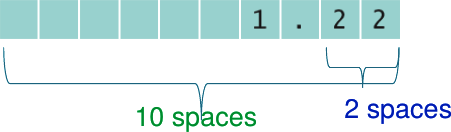
\includegraphics[height=0.15\paperheight,left]{pucrs-ep-fprog-unidade_02-tipos_de_dados_fundamentais-laminas-formatacao.png}
\end{figure}
	\item \texttt{\%.2f} e \texttt{\%10.2f} são especificadores de formato
\end{itemize}
\end{frame}

%-------------------------------------------------------
\begin{frame}[fragile]\frametitle{Tipos de Formatação}
\begin{itemize}
	\item A formatação é bastante útil para alinhar colunas na saída
{\footnotesize
\begin{center}
\begin{tikzpicture}
\node[drop shadow,fill=white,inner sep=0pt] 
{\rowcolors{1}{RoyalBlue!20}{RoyalBlue!5}
  \begin{tabular}{|C{1.5cm}|C{8cm}|l|}
\hline
    \textbf{Código}  & \textbf{Tipo} & \textbf{Exemplo}\\
\hline
    \texttt{d} & Inteiros decimais & \texttt{123} \\
    \texttt{f} & Ponto-flutuante fixo & \texttt{12.30} \\
    \texttt{e} & Ponto-flutuante exponencial & \texttt{1.23e+1} \\
    \texttt{g} & Ponto-flutuante genérico (notação exponencial será usada para números muito grandes ou muito pequenos) & \texttt{12.3} \\
    \texttt{s} & Cadeias de caracteres (\emph{strings}) & \texttt{Tax:} \\
\hline
  \end{tabular}
};
\end{tikzpicture}
\end{center}
}
	\item Você também pode incluir texto dentro das aspas:
\begin{javacode}
System.out.printf("Preco por litro: %10.2f", price);
\end{javacode}
	\item Ou incluir mais de um especificador de formato dentro das aspas e quebras de linha (\texttt{\textbackslash}):
\begin{javacode}
System.out.printf("As raizes sao: %10.4f e %10.4f\n", x1,x2);
\end{javacode}
\end{itemize}
\end{frame}

%-------------------------------------------------------
\begin{frame}\frametitle{Modificadores de Formatação}
\begin{itemize}
	\item Você também pode usar modificadores de formatação para alterar o modo como valores numéricos e textos são exibidos
{\footnotesize
\begin{center}
\begin{tikzpicture}
\node[drop shadow,fill=white,inner sep=0pt] 
{\rowcolors{1}{RoyalBlue!20}{RoyalBlue!5}
  \begin{tabular}{|c|l|l|}
\hline
    \textbf{Modificador}  & \textbf{Significado} & \textbf{Exemplo}\\
\hline
    \texttt{-} & Alinhamento à esquerda & \texttt{1.23} (seguido por espaços) \\
    \texttt{0} & Preenchimento com zeros & \texttt{001.23} \\
    \texttt{+} & Mostra o sinal também para números positivos & \texttt{+1.23} \\
\hline
  \end{tabular}
};
\end{tikzpicture}
\end{center}
}
\end{itemize}
\end{frame}

%-------------------------------------------------------
\begin{frame}[fragile]\frametitle{Exemplos de Modificadores de Formatação}
\begin{itemize}
	\item Alinhamento à esquerda de um \emph{string}:
\begin{javacode}
System.out.printf("%-10s", "Total:");
\end{javacode}
\begin{figure}[h]
	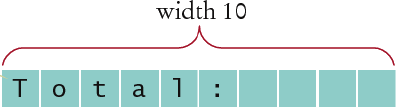
\includegraphics[height=0.14\paperheight,left]{pucrs-ep-fprog-unidade_02-tipos_de_dados_fundamentais-laminas-formatacao2.png}
\end{figure}
	\item Alinhamento à direita de um número com 2 casas decimais:
\begin{javacode}
System.out.printf("%10.2f", price);
\end{javacode}
\begin{figure}[h]
	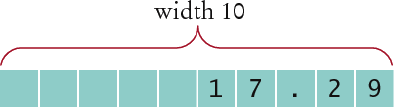
\includegraphics[height=0.14\paperheight,left]{pucrs-ep-fprog-unidade_02-tipos_de_dados_fundamentais-laminas-formatacao3.png}
\end{figure}
\end{itemize}
\end{frame}

%-------------------------------------------------------
\begin{frame}[fragile]\frametitle{Exemplos de Modificadores de Formatação}
\begin{itemize}
	\item Impressão de múltiplos valores:
\begin{javacode}
System.out.printf("%-10s%10.2f", "Total:", price);
\end{javacode}
\begin{figure}[h]
	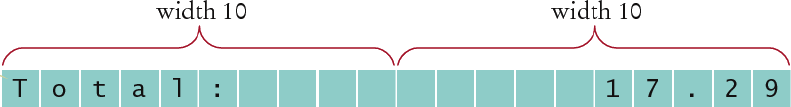
\includegraphics[height=0.15\paperheight,left]{pucrs-ep-fprog-unidade_02-tipos_de_dados_fundamentais-laminas-formatacao1.png}
\end{figure}
\end{itemize}
\end{frame}

%-------------------------------------------------------
\begin{frame}[fragile]\frametitle{\texttt{Volume2.java} {\tiny (HORSTMANN, 2013, p. 51-52)}}
{\tiny
\begin{javacode}
import java.util.Scanner;

/**
   This program prints the price per ounce for a six-pack of cans.
*/
public class Volume2 {
   public static void main(String[] args) {
      // Read price per pack
      Scanner in = new Scanner(System.in);
      System.out.print("Please enter the price for a six-pack: ");
      double packPrice = in.nextDouble();

      // Read can volume
      System.out.print("Please enter the volume for each can (in ounces): ");
      double canVolume = in.nextDouble();

      // Compute pack volume
      final double CANS_PER_PACK = 6;
      double packVolume = canVolume * CANS_PER_PACK;

      // Compute and print price per ounce
      double pricePerOunce = packPrice / packVolume;
      System.out.printf("Price per ounce: %8.2f", pricePerOunce);
      System.out.println();
   }
}
\end{javacode}
}
\end{frame}

%-------------------------------------------------------
\begin{frame}\frametitle{Documentação da API Java}
\begin{itemize}
	\item A lista de classes e métodos da API Java pode ser obtida em: \url{http://docs.oracle.com/javase/8/docs/api/}
\begin{figure}[h]
	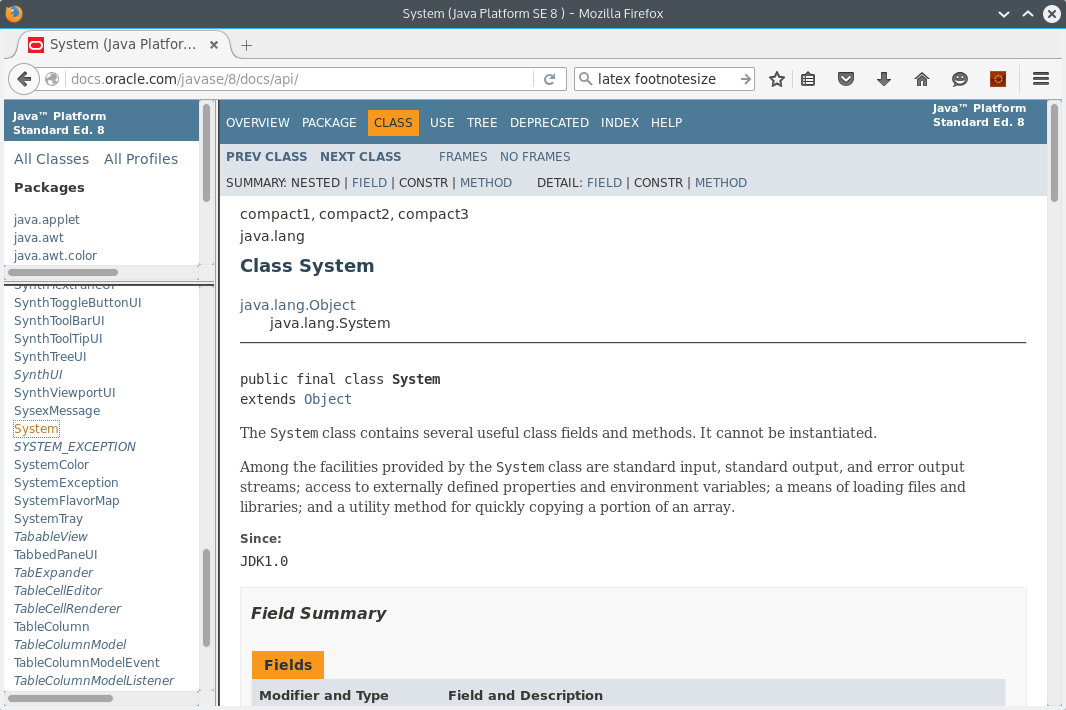
\includegraphics[height=0.6\paperheight,center]{pucrs-ep-fprog-unidade_02-tipos_de_dados_fundamentais-laminas-api_java.jpg}
\end{figure}
\end{itemize}
\end{frame}

%=======================================================
\section{Resolução de Problemas: Primeiro Faça à Mão}

%-------------------------------------------------------
\begin{frame}\frametitle{Resolução de Problemas: Primeiro Faça à Mão}
\begin{itemize}
	\item Um passo bastante importante para desenvolver um algoritmo é primeiro realizar as computações à mão.
	\item Por exemplo:
	\begin{itemize}
		\item Uma linha de azulejos pretos e brancos deve ser colocada ao longo de uma parede. Por razões estéticas, o arquiteto especificou que o primeiro e o último bloco devem ser pretos.
		\item Sua tarefa é computar o número de azulejos necessários e o espaço de sobra em cada extremidade, dado o espaço disponível e o comprimento de cada azulejo.
\begin{figure}[h]
	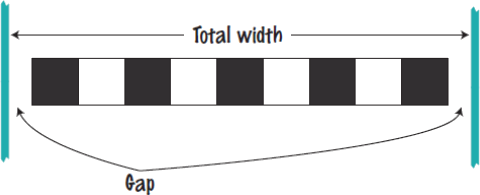
\includegraphics[height=0.25\paperheight,center]{pucrs-ep-fprog-unidade_02-tipos_de_dados_fundamentais-laminas-exemplo_a_mao.png}
\end{figure}
	\end{itemize}
\end{itemize}
\end{frame}

%-------------------------------------------------------
\begin{frame}\frametitle{Inicie com exemplos de teste}
\begin{itemize}
	\item Valores iniciais de teste
	\begin{itemize}
		\item Espaço total: $1000cm$
		\item Tamanho de cada azulejo: $50cm$
	\end{itemize}
	\item Teste seus valores
	\begin{itemize}
		\item Vejamos... $1000cm/50cm = 20$, perfeito! $20$ azulejos. Nenhuma sobra.
		\item Mas, espere... Preto, Branco; Preto, Branco; ... "O primeiro e o último azulejo devem ser pretos."
	\end{itemize}
	\item Olhe mais atentamente para o problema...
	\begin{itemize}
		\item Inicie com um azulejo preto, então some determinado número de pares de azulejos branco-preto
\begin{figure}[h]
	
\includegraphics[height=0.05\paperheight,center]{pucrs-ep-fprog-unidade_02-tipos_de_dados_fundamentais-laminas-exemplo_a_mao2.png}
\end{figure}
		\item Observação: cada par tem 2 vezes o tamanho de um azulejo (em nosso exemplo: $2 \times 50cm = 100cm$)
	\end{itemize}
\end{itemize}
\end{frame}

%-------------------------------------------------------
\begin{frame}\frametitle{Continue Trabalhando na sua Solução}
\begin{itemize}
	\item Calcule o comprimento total dos azulejos
	\begin{itemize}
		\item Um azulejo preto: $50cm$
		\item 9 pares de azulejos branco-preto: $900cm$
		\item Comprimento total: $950cm$
	\end{itemize}
	\item Cálculo da sobra (uma em cada extremidade):
	\begin{itemize}
		\item $1000cm - 950cm = 50cm$ de sobra total
		\item $50cm / 2 = 25cm$ em cada extremidade
	\end{itemize}
\end{itemize}
\end{frame}

%-------------------------------------------------------
\begin{frame}\frametitle{Agora Pense no Algoritmo}
\begin{itemize}
	\item Use o exemplo para ver como os valores foram calculados
	\item Quantos pares? (deve ser um número inteiro)\\
		\texttt{numPares = (int) (compTotal - compAzulejo) / (2 $\times$ compAzulejo)}
	\item Quantos azulejos?\\
		\texttt{numAzulejos = 1 + 2 $\times$ numPares}
	\item Sobra em cada extremidade?\\
		\texttt{sobra = (compTotal - numAzulejos $\times$ compAzulejo) / 2}
\end{itemize}
\end{frame}

%-------------------------------------------------------
\begin{frame}\frametitle{Exercício}
Considere um terreno retangular sobre o qual se deseja colocar ``placas'' de grama que são vendidas por metro quadrado. Neste terreno há um silo redondo e uma casa em formato retangular. Determine os dados que devem ser lidos para que se saiba o custo da colocação de grama nesse terreno e faça o programa em Java para realizar este cálculo.
\begin{figure}[h]
	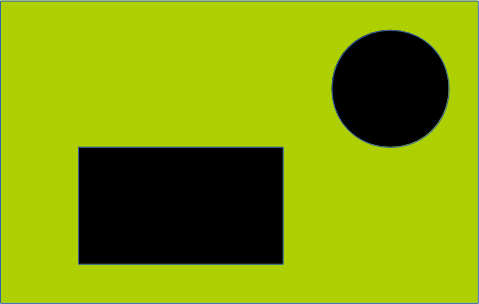
\includegraphics[height=0.25\paperheight,center]{pucrs-ep-fprog-unidade_02-tipos_de_dados_fundamentais-laminas-problema.png}
\end{figure}
\end{frame}

%=======================================================
\section{Cadeias de Caracteres (Strings)}

%-------------------------------------------------------
\begin{frame}[fragile]\frametitle{\emph{Strings}}
\begin{itemize}
	\item O tipo \texttt{String} é usado para armazenamento de textos (sequências de caracteres)
	\item Sintaxe:
{\small
\begin{javacode}
// <tipo> <nome variavel> = <conteudo inicial> ;
String nome = "Texto";
\end{javacode}
}
	\item Uma vez que você tenha uma variável do tipo \texttt{String}, você pode usar métodos como:
{\small
\begin{javacode}
int n = nome.length(); // n recebera o valor 5
\end{javacode}
}
	\item O comprimento de um \emph{string} corresponde ao número de caracteres que ele contém
	\begin{itemize}
		\item Um \emph{string} vazio (tamanho 0) corresponde a \texttt{"}\texttt{"}
		\item O tamanho máximo de um \emph{string} é bastante grande (um \texttt{int})
	\end{itemize}
\end{itemize}
\end{frame}

%-------------------------------------------------------
\begin{frame}[fragile]\frametitle{Concatenação de \emph{Strings} (\texttt{+})}
\begin{itemize}
	\item Você pode ``adicionar'' um \emph{string} no final de outro:
{\scriptsize
\begin{javacode}
String pNome = "Joao";
String uNome = "Silva";
String nome = pNome + uNome; // JoaoSilva
\end{javacode}
}
	\item Quer um espaço entre os nomes?
{\scriptsize
\begin{javacode}
String nome = pNome + " " + uNome; // Joao Silva
\end{javacode}
}
	\item Para concatenar uma variável numérica a um \emph{string}:
{\scriptsize
\begin{javacode}
String a = "Agente";
int n = 7;
String bond = a + n; // Agente7
\end{javacode}
}
	\item Concatenar \emph{strings} e números em \texttt{println}:
{\scriptsize
\begin{javacode}
System.out.println("Total = " + total);
\end{javacode}
}
\end{itemize}
\end{frame}

%-------------------------------------------------------
\begin{frame}[fragile]\frametitle{Entrada de \emph{Strings}}
\begin{itemize}
	\item Você pode ler um \emph{string} do terminal com \texttt{next}
	\begin{itemize}
		\item O método \texttt{next} lê uma palavra de cada vez
		\item Palavras lidas por \texttt{next} são separadas por espaços
	\end{itemize}
{\scriptsize
\begin{javacode}
System.out.print("Digite seu primeiro nome: ");
String nome = in.next();
\end{javacode}
}
	\item Você pode ler uma linha inteira do terminal com \texttt{nextLine}
	\begin{itemize}
		\item O método \texttt{nextLine} faz a leitura até encontrar um ``Enter''
	\end{itemize}
{\scriptsize
\begin{javacode}
System.out.print("Forneca o seu endereco: ");
String endereco = in.nextLine();
\end{javacode}
}
	\item Para converter uma variável \texttt{String} para um número:
{\scriptsize
\begin{javacode}
System.out.print("Digite a sua idade: ");
String entrada = in.nextLine();
int idade = Integer.parseInt(entrada); // apenas digitos
\end{javacode}
}
\end{itemize}
\end{frame}

%-------------------------------------------------------
\begin{frame}[fragile]\frametitle{Sequências de Escape em \emph{Strings}}
\begin{itemize}
	\item Como imprimir aspas duplas?
	\begin{itemize}
		\item Coloque uma \texttt{\textbackslash} antes do \texttt{"}, dentro do \emph{string}
	\end{itemize}
\begin{javacode}
System.out.print("Ele disse \"Alo\"");
\end{javacode}
	\item Ok, e agora como imprimir uma contra-barra?
	\begin{itemize}
		\item Coloque uma \texttt{\textbackslash} antes da \texttt{\textbackslash}!
	\end{itemize}
\begin{javacode}
System.out.print("C:\\Temp\\Secret.txt");
\end{javacode}
	\item Mude de linha dentro de um \emph{string} (\texttt{\textbackslash}\texttt{n}):
\begin{javacode}
System.out.print("*\n**\n***\n");
\end{javacode}
\end{itemize}
\end{frame}

%-------------------------------------------------------
\begin{frame}[fragile]\frametitle{\emph{Strings} e Caracteres}
\begin{itemize}
	\item \emph{Strings} são sequências de caracteres
	\begin{itemize}
		\item Caracteres \emph{Unicode}, para ser mais exato
		\item Caracteres tem seu próprio tipo: \texttt{char}
		\item Caracteres têm valores numéricos
		\begin{itemize}
			\item Consulte uma tabela ASCII para descobrir o valor de cada código
			\item Por exemplo, a letra 'A' teria o valor 65 se fosse um número
		\end{itemize}
	\end{itemize}
	\item Usa-se apóstrofos ao redor de caracteres:
\begin{javacode}
char initial = 'B';
\end{javacode}
	\item Usa-se aspas ao redor de \emph{strings}:
\begin{javacode}
String initials = "BRL";
\end{javacode}
\end{itemize}
\end{frame}

%-------------------------------------------------------
\begin{frame}[fragile]\frametitle{Obtendo um caracter de um \emph{String}}
\begin{itemize}
	\item Cada caracter dentro de um \emph{string} tem um índice numérico
	\item O primeiro caracter tem o índice $0$
	\item O método \texttt{charAt} retorna o caracter com determinado índice em um \emph{string}
\begin{javacode}
String nome = "Harry";
char inicio = nome.charAt(0);
char fim = nome.charAt(4);
\end{javacode}
\begin{figure}[h]
	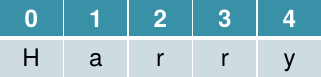
\includegraphics[height=0.1\paperheight,center]{pucrs-ep-fprog-unidade_02-tipos_de_dados_fundamentais-laminas-string.png}
\end{figure}
\end{itemize}
\end{frame}

%-------------------------------------------------------
\begin{frame}[fragile]\frametitle{Obtendo uma Parte de um \emph{String}}
\begin{itemize}
	\item Um \emph{substring} é uma parte de um \emph{string}
	\item O método \texttt{substring(índice inicial,limite final)} retorna um conjunto de caracteres a partir de uma posição (índice inicial) de um \emph{string}
\begin{javacode}
String greeting = "Hello!";
String sub = greeting.substring(0, 2);  // = "He"
String sub2 = greeting.substring(3, 5); // = "lo"
\end{javacode}
\end{itemize}
\end{frame}

%-------------------------------------------------------
\begin{frame}[fragile]\frametitle{Obtendo uma Parte de um \emph{String}}
{\scriptsize
\begin{javacode}
public class TesteDeSubstring {
    public static void main (String args[])
    {
        String texto = "01234";
        System.out.println("["+texto.substring(0)+"]");   // [01234]
        System.out.println("["+texto.substring(1)+"]");   // [1234]
        System.out.println("["+texto.substring(2)+"]");   // [234]
        System.out.println("["+texto.substring(3)+"]");   // [34]
        System.out.println("["+texto.substring(4)+"]");   // [4]
        System.out.println("["+texto.substring(5)+"]\n"); // []
        /* ERRO DE EXECUCAO:
        System.out.println("["+texto.substring(1,0)+"]"); */
        System.out.println("["+texto.substring(1,1)+"]"); // []
        System.out.println("["+texto.substring(1,2)+"]"); // [1] 
        System.out.println("["+texto.substring(1,3)+"]"); // [12]
        System.out.println("["+texto.substring(1,4)+"]"); // [123]
        System.out.println("["+texto.substring(1,5)+"]"); // [1234]
    }
}
\end{javacode}
}
\end{frame}

%-------------------------------------------------------
\begin{frame}\frametitle{Operações sobre \emph{Strings}}
\begin{figure}[h]
	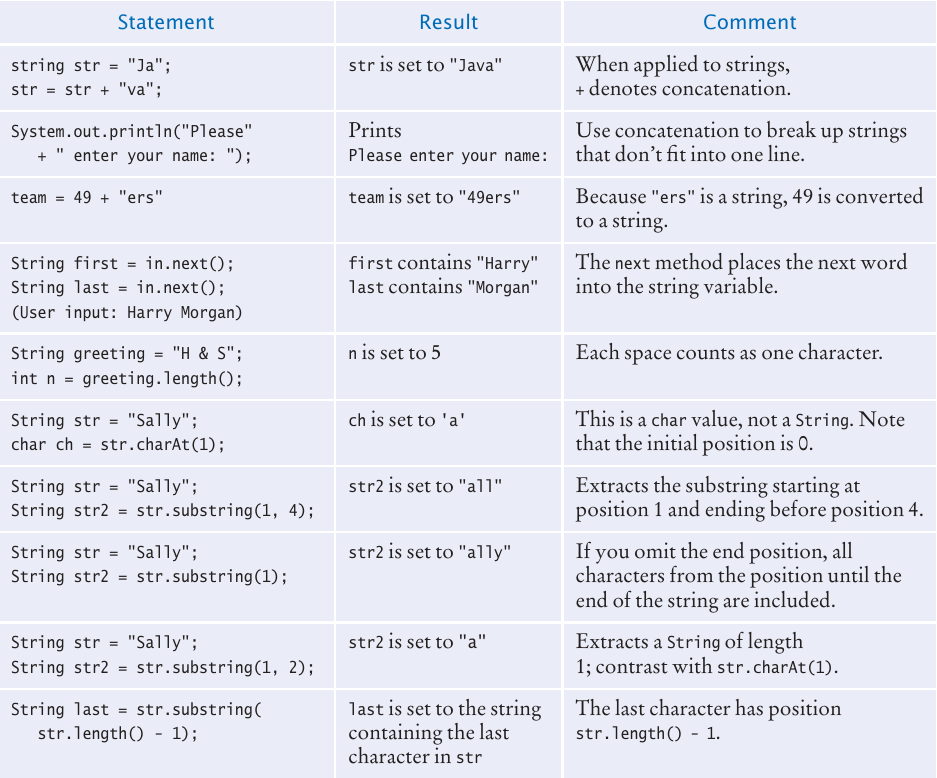
\includegraphics[height=0.7\paperheight,center]{pucrs-ep-fprog-unidade_02-tipos_de_dados_fundamentais-laminas-operacoes_sobre_strings.png}
\end{figure}
\end{frame}

%-------------------------------------------------------
\begin{frame}\frametitle{Principais métodos de \emph{String} (1)}
\begin{itemize}
\item \texttt{char charAt(int index)}: retorna o valor do caractere no índice especificado
\item \texttt{int compareTo(String anotherString)}: comparação lexicográfica (diferenciando caixa alta e caixa baixa)
\item \texttt{int compareToIgnoreCase(String str)}: comparação lexicográfica (ignornado caixa alta e caixa baixa)
\item \texttt{String concat(String str)}: concatena a \emph{string} especificada no final desta \emph{string}
\item \texttt{boolean endsWith(String suffix)}: verifica se a \emph{string} termina com o sufixo especificado
\item \texttt{boolean equals(Object anObject)}: verifica se a \emph{string} especificada é igual a esta
\item \texttt{boolean equalsIgnoreCase(String anotherString)}: verifica se a \emph{string} especificada é igual a esta, sem diferenciar caixa alta e caixa baixa
\end{itemize}
\end{frame}

%-------------------------------------------------------
\begin{frame}\frametitle{Principais métodos de \emph{String} (2)}
\begin{itemize}
\item \texttt{int hashCode()}: retorna um \emph{hash code} para esta \emph{string}
%int indexOf(int ch)
%Returns the index within this string of the first occurrence of the specified character.
%int indexOf(int ch, int fromIndex)
%Returns the index within this string of the first occurrence of the specified character, starting the search at the specified index.
%int indexOf(String str)
%Returns the index within this string of the first occurrence of the specified substring.
%int indexOf(String str, int fromIndex)
%Returns the index within this string of the first occurrence of the specified substring, starting at the specified index.
%String intern()
%Returns a canonical representation for the string object.
\item \texttt{boolean isEmpty()}: retorna \texttt{true} se, e somente se, o \texttt{length()} for igual a 0
%int lastIndexOf(int ch)
%Returns the index within this string of the last occurrence of the specified character.
%int lastIndexOf(int ch, int fromIndex)
%Returns the index within this string of the last occurrence of the specified character, searching backward starting at the specified index.
%int lastIndexOf(String str)
%Returns the index within this string of the last occurrence of the specified substring.
%int lastIndexOf(String str, int fromIndex)
%Returns the index within this string of the last occurrence of the specified substring, searching backward starting at the specified index.
\item \texttt{int length()}: retorna o tamanho desta \emph{string}
%Returns the length of this string.
%boolean matches(String regex)
%Tells whether or not this string matches the given regular expression.
%int offsetByCodePoints(int index, int codePointOffset)
%Returns the index within this String that is offset from the given index by codePointOffset code points.
%boolean regionMatches(boolean ignoreCase, int toffset, String other, int ooffset, int len)
%Tests if two string regions are equal.
%boolean regionMatches(int toffset, String other, int ooffset, int len)
%Tests if two string regions are equal.
%String replace(char oldChar, char newChar)
%Returns a new string resulting from replacing all occurrences of oldChar in this string with newChar.
%String replace(CharSequence target, CharSequence replacement)
%Replaces each substring of this string that matches the literal target sequence with the specified literal replacement sequence.
%String replaceAll(String regex, String replacement)
%Replaces each substring of this string that matches the given regular expression with the given replacement.
%String replaceFirst(String regex, String replacement)
%Replaces the first substring of this string that matches the given regular expression with the given replacement.
%String[] split(String regex)
%Splits this string around matches of the given regular expression.
%String[] split(String regex, int limit)
%Splits this string around matches of the given regular expression.
%boolean startsWith(String prefix)
%Tests if this string starts with the specified prefix.
%boolean startsWith(String prefix, int toffset)
%Tests if the substring of this string beginning at the specified index starts with the specified prefix.
%CharSequence subSequence(int beginIndex, int endIndex)
%Returns a new character sequence that is a subsequence of this sequence.

\item \texttt{String substring(int beginIndex)}: retorna uma nova \emph{string} que é uma \emph{substring} desta \emph{string}, do índice até o final
\item \texttt{String substring(int beginIndex, int endIndex)}: retorna uma nova \emph{string} que é uma \emph{substring} desta \emph{string}
\end{itemize}
\end{frame}

%-------------------------------------------------------
\begin{frame}\frametitle{Principais métodos de \emph{String} (3)}
\begin{itemize}
\item \texttt{String toLowerCase()}: converte todos os caracteres desta \emph{string} para uma \emph{string} em caixa baixa usando as regras da localidade padrão
\item \texttt{String toLowerCase(Locale locale)}: converte todos os caracteres desta \emph{string} para uma \emph{string} em caixa baixa usando as regras da localidade especificada
\item \texttt{String toString()}: este objeto (que já é uma \emph{string}) é autoretornado
\item \texttt{String toUpperCase()}: converte todos os caracteres desta \emph{string} para uma \emph{string} em caixa alta usando as regras da localidade padrão
\item \texttt{String toUpperCase(Locale locale)}: converte todos os caracteres desta \emph{string} para uma \emph{string} em caixa alta usando as regras da localidade especificada
\end{itemize}
\end{frame}

%-------------------------------------------------------
\begin{frame}\frametitle{Principais métodos de \emph{String} (4)}
\begin{itemize}
\item \texttt{String trim()}: retorna uma cópia da \emph{string} eliminando espaços iniciais e finais
\item \texttt{static String valueOf(boolean b)}: retorna uma \emph{string} represesntando o argumento \texttt{boolean}
\item \texttt{static String valueOf(char c)}:  retorna uma \emph{string} represesntando o argumento \texttt{char}
\item \texttt{static String valueOf(double d)}:  retorna uma \emph{string} represesntando o argumento \texttt{double}
\item \texttt{static String valueOf(float f)}:  retorna uma \emph{string} represesntando o argumento \texttt{float}
\item \texttt{static String valueOf(int i)}:  retorna uma \emph{string} represesntando o argumento \texttt{int}
\item \texttt{static String valueOf(long l)}:  retorna uma \emph{string} represesntando o argumento \texttt{long}

\item ...

\end{itemize}
\end{frame}

%=======================================================
\section{Referências}

%-------------------------------------------------------
\begin{frame}\frametitle{Referências}
\noindent{HORSTMANN, C. \textbf{Java for Everyone – Late Objetct}. 2. ed. Hoboken: Wiley, 2013. xxxiv, 589 p.}
\end{frame}

%=======================================================
\end{document}

